\documentclass[prl,twocolumn,showpacs]{revtex4}

\usepackage{epsfig,color,graphicx,amsmath}
\begin{document}
\newcommand{\Ang}{\ensuremath{\mathring{\text{A}}}}
\newcommand{\ltwid}{\mathrel{\raise.3ex\hbox{$<$\kern-.75em\lower1ex\hbox{$\sim$}}}}
\newcommand{\gtwid}{\mathrel{\raise.3ex\hbox{$>$\kern-.75em\lower1ex\hbox{$\sim$}}}}
\newcommand{\bra}{\langle}
\newcommand{\ket}{\rangle}
%\newcommand{\sill}{\psi_\mathrm{SILL}}
\newcommand{\sill}{\psi}
\newcommand{\trace}{{\rm Tr}}
\newcommand{\ntilde}{\tilde{n}}
\newcommand{\stilde}{\tilde{s}}
\newcommand{\atilde}{\tilde{\alpha}}
\newcommand{\new}{\color{red}}
\newcommand{\old}{\color{black}}
\newcommand{\bea}{\begin{eqnarray}}
\newcommand{\eea}{\end{eqnarray}}
\newcommand{\br}{\ensuremath{\mathbf{r}}}
\def\nn{\nonumber\\}

\bibliographystyle{apsrev}

\title{Linear scaling density functional method based on localized molecular orbits}

\author{Yifei Shi}
\affiliation{Department of Chemistry, McGill University, 801 Sherbrooke St. West, Montreal, QC H3A 0B8, Canada}

\author{Rustam Z. Khaliullin}
\affiliation{Department of Chemistry, McGill University, 801 Sherbrooke St. West, Montreal, QC H3A 0B8, Canada}

%\date{\today}

\begin{abstract}
Density functional theory based on localized molecular orbits are known to have convergence issues. In this work, we develop a new method that avoids the problem by modifying the preconditioned conjugate gradient method. The optimization directions causing the slow convergence is filtered out and neglected using the approximate Hessian. We show that, by removing these directions, the energy and other properties can be obtained accurately and the computational cost is significantly reduced. This corresponds to posing a relaxed orthogonality constrains on the molecuar orbits. We demonstrate the efficiency of the method on systems from molecular systems to semi-conductors. Furthermore, although this method is not fully variational, it is still accurate enough to produce stable molecular dynamics in systems where chemical reactions happen.

\end{abstract}
\maketitle

\emph{Introduction} 
The Kohn-Sham formulism of density functional theory (DFT)\cite{hohenberg1964inhomogeneous,kohn1965self} has been the most efficient and successful tool in electronic structure calculations. However, the cubic scaling ($\sim N$) of computational cost prevents its application in large systems of interest. To overcome the limit of Kohn-Sham DFT, recent reaserch interest has focused on the development of linearly scaling (LS) DFT methods\cite{bowler2012methods,goedecker1999linear}. 

All LS DFT method utilize the localized nature of gapped systems. A large family of methods work with the one-electron density matrix (DM)\cite{li1993density,lee1996linear,li2003density,vandevondele2012linear}, $F(\mathbf{r},\mathbf{r}^{'})=\sum_i f_i \phi_i(\mathbf{r}) \phi_i(\mathbf{r}^{'})$, which decays exponentially in $|\mathbf{r}-\mathbf{r}^{'}|$.These include methods like the Fermi operator expansion\cite{goedecker1994efficient,goedecker1995tight}, divide-and-conquer method\cite{yang1991direct,yang1991local}, and density matrix minimization method\cite{li1993density}. However, in a typical electronic structure calculation, the number of atomic orbits (AOs) is much larger than the number of molecular orbits (MOs), thus DM methods generally need to handle larger matrices and more variational parameters, limiting the DM methods mostly to minimal-basis tight-binding problems. 

Another approach to LS DFT is based on local molecular orbits (LMO), where electrons can only occupy AOs of certain molecules. Since in general locality and orthogonality is not simultaneously obtainable, non-orthogonal LMOs are generally used. To avoid the calculation of the inverse of MO overlap matrix, a series of work have focused on using new energy functionals \cite{mauri1993orbital,kim1995total,ordejon1995linear}, or introducing extra optimization variables \cite{burger2008linear,peng2013effective}. This approach has the advantage of being more intuitive and containing relatively fewer variational parameters, it can also provide useful information about the charge transfer interaction \cite{khaliullin2007unravelling,khaliullin2008analysis}. However, the LMO approach suffers from intrinsic convergence problems\cite{ordejon1995linear,fattebert2004linear}. Several efforts were made to deal with this problem. In \cite{tsuchida2007augmented,tsuchida2008ab}, the MOs are forced to be orthogonal to an auxiliary wave function on a ``kernel region". Recently, in \cite{khaliullin2013efficient}, a block-diagonal reference is first calculated and then corretion which is constrained to be orthogonal to the reference is added in the second step. These two methods have all been successful in improving the convergence by constraining the MOs to be orthogonal to some reference states, thus requiring the reference to be somewhat physically meaningful.

Furthermore, we notice that the LMO approach may lead to a ground state that suffers from orbital collapsing. This is illustrated by a straight forward energy minimization of a simple systems with 4 HF molecules. We used DZVP basis set and preconditioned conjugate gradient algorithm. In Fig ~\ref{fig:det} we show the determinant of the MO overlap matrix and the maximum norm of the energy gradient as a function of the minimization step. The minimization brings the state into a singular point and as a result the energy gradient does not vanish. This aggravates the convergence problem.

\begin{figure}
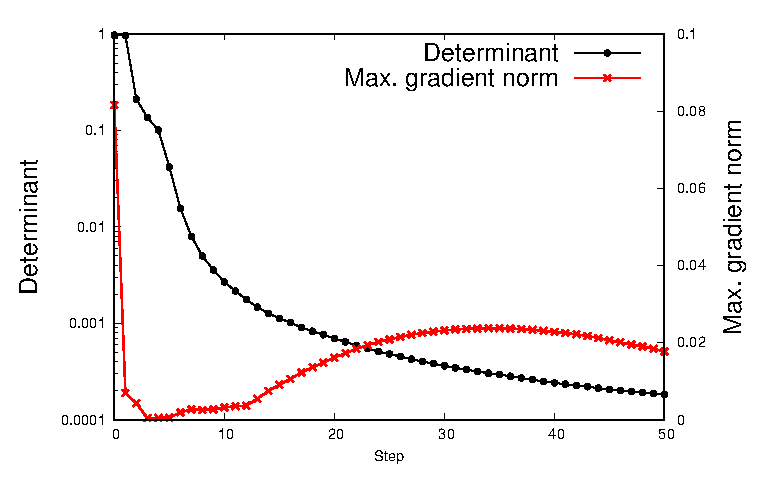
\includegraphics[width=0.5\textwidth]{det}
\caption{The determinant of the MO overlap matrix, and maximum norm of the energy gradient. }
\label{fig:det}
\end{figure}
%Furthermore it was also shown in \cite{ordejon1995linear} that the straight forward LMO calculation without using a new energy functional may end up in a set of MOs that are collapsing. And the new energy functionals may lead to multiple minima \cite{kim1995total}.

Despite the rapid development in LS DFT, a reliable method is still lacking for large and strong interacting systems. In this work, we develop a new LS DFT method, based on LMOs, by identifying and filtering out the optimization directions that cause the slow convergence. We call it Hessian filter method and it has the advantage that: (a) The energy converges fast, and works with systems where interactions are strong. (b) No ``block-diagonal reference" or ``kernel region" are needed like in \cite{tsuchida2007augmented} or \cite{khaliullin2013efficient}.
%(b) The problem of orbital collapse is avoided. (c) Exact inverse of the MO overlap matrix is used, the inversion is linear when the overlap is sparse. This prevents the error introduced by approximate inverse overlap and the problem of multiple minima. 
(c) The problem of orbital collapse is avoided. (d) Although this method is not fully variational and the energy is not the minimum of any energy functional, it still produces stable dynamics for systems involving chemical reactions. 

\emph{Theory}
In the LMO approach electrons are seperated into fragments, which in most cases are molecules. Each fragment has certain geometrically neighboring fragments within a cutoff radii $R_c$, and electron MOs on this fragment can only occupy AOs on the neighboring fragments, these orbits are expected to represent the maximally localized Wannier functions \cite{marzari1997maximally,he2001exponential}. In this work, fragments are denoted by $x,y..$, AOs are denoted by greek letters $\chi_\mu,\chi_\nu ..$, MOs are denoted by $\psi_i,\psi_j..$, $\chi_{x\mu}$ denotes the AOs which electrons in fragment $x$ can occupy. In this paper, the orbital indices are summed over but not fragment indices. Then MO $i$ in fragment $x$ can be expressed as:
\bea
\psi_{xi} = |\chi_{x\mu}\rangle T^{x\mu}_{\quad xi}
\label{eq:LMO}
\eea

The AO to MO matrix $T$ thus has blocked form, and the identity operator on fragment $x$ is:

\bea
\hat{\mathbf{I}}_x = |\chi_{x\mu}\rangle S^{x\mu,x\nu} \langle \chi_{x\nu} |
\eea

where $S^{x\mu,x\nu}$ is the matrix element of the inverse overlap matrix $S_{x\mu,x\nu}$. Consider the DFT energy functional:

\bea
E[\{\psi_i\}] &=& 2\sum_{i,j} (\sigma^{-1})_{i,j}\int \psi_i(\br) (-\frac{1}{2}\nabla^2) \psi_j(\br)d\br \nonumber \\
&+& \frac{1}{2} \int \int \frac{\rho(\br)\rho(\br')}{|\br-\br'|}d\br d\br' + E_{XC}[\rho] \\
&+& 2\sum_{i,j} (\sigma^{-1})_{i,j}\int \psi_i(\br) V_{ext}({\br}) \psi_j(\br) d\br \nonumber
\eea

A straight forward minimization of the energy functional will lead to the aforementioned slow convergence and orbital collapse problems, and can be understood by the following analysis. We define an operator $P^x$ for each fragment $x$ where:

\bea
P^x |\chi_\mu\rangle = \begin{cases}
|\chi_\mu\rangle &\mu \text{ is an AO on fragment } x \\
0 & \text{otherwise}
\end{cases}
\eea

The introduction of local constrains in Eq~(\ref{eq:LMO}) destroys the strict invariance of energy under unitary tranformations of occupied MOs, and only unitary transformations within a certain fragment leaves the energy exactly invariant. This can been understood by consider 2 MOs in fragments $x$ and $y$, $\psi_{xi}=|\chi_{x\mu}\rangle T^{x\mu}_{\quad xi}$, $\psi_{yj}=|\chi_{y\nu}\rangle T^{y\nu}_{\quad yj}$, since they two fragments have different sets of AOs associated with them, mixing of these two MOs will break the localization constrain and is thus forbidden. However, approximate invariance can still exist in certain directions where the energy changes very slowly. This corresponds to a mixing of the form:

\bea
\psi_{xi} \rightarrow \alpha\psi_{xi} + \beta P^x\psi_{yj}
\label{eq:baddir}
\eea

where $\alpha$ and $\beta$ are two transformation coefficients. $P^x$ ensures that the resulting orbit still satisfies the localization constrain. In the case that $x$ and $y$ fragments are neighbors, this operation may only slightly change the orbits in $y$, and thus the energy.

These directions are the heart of the convergence problems concerning the calculations based on LMOs\cite{goedecker1999linear}. We propose to solve the problem by identifying the ``bad" directions via the Hessian and design a optimization scheme that avoids these directions completely. We also comment on the physical meaning of these bad directions.

To proceed, consider in a normal preconditioned conjugate gradient (PCG) procedure, the energy gradient is given by:

\bea
G^{\quad xi}_{x\mu} = 4[(\mathbf{I}-SR)fT\sigma^{-1}]^{\quad xi}_{x\mu}
\eea

 we consider the approximate Hessian\cite{stoll1980use},

\small{
\bea
Hess^{xi,yj}_{x\mu,x\nu} &=& \frac{\partial^2 E}{\partial T^{x\mu}_{\quad xi} \partial T^{y\nu}_{\quad yj}} \nonumber \\
&\approx& \delta_{xy}[(I_x-S^xR^x)f(I^x-R^xS^x) \nonumber \\
&+& (I_x - S^xR^xS^x)]_{x\mu,x\nu} 
\label{eq:hess}
\eea
}
where $S^x = P^x \cdot S \cdot P^x$ and $R^x = P^x \cdot R \cdot P^x$ are the projection of the overlap matrix and density matrix on fragment x. This is a good approximation close to the energy minima. This Hessian has blocked form, and contains one matrix for each fragment, which will be denoted by $Hess^{[x]}$. The eigenvalues and eigenvectors of the Hessian contain information about the direction of optimization: occupied-virtual mixing corresponds to large eigenvalues, occupied-occupied mixing within a fragment corresponds to exactly zero eigenvalues, and the bad directions correspond to small but none-zero eigenvalues. However, because of the tensorial properties of the Hessian, we must solve the generalized eigen problem instead:

\bea
(S^x)^{-\frac{1}{2}} Hess^{[x]} (S^x)^{-\frac{1}{2}} (S^x)^{\frac{1}{2}} A^x =  (S^x)^{\frac{1}{2}} A^x \Lambda
\label{eq:gev}
\eea

where the columns $A^x$ contain the eigenvectors of $Hess^{[x]}$ and $\Lambda$ is a positive semidefinite diagonal matrix\cite[??].
We define a projector:

\bea
Q^x = (A^x)^T \Theta A^x \label{eq:qx}
\eea

where $\Theta$ is a diagonal matrix whose diagonal elements are 0 if the eigen vector is considered bad and need to be removed, and 1 otherwise. So $Q^x$ is the operator the filters out the directions causes the slow optimization. We then define a new gradient and preconditioner that have correct tensorial properties:

\bea
\bar{G}^x &=& (S^x)^{\frac{1}{2}} Q^x (S^x)^{-\frac{1}{2}} G^x \nonumber \\
\bar{Prec}^x &=& (S^x)^{-\frac{1}{2}} Q^x (S^x)^{\frac{1}{2}} {Prec}^x
\eea

where $G^x$ and ${Prec}^x = (Hess^x)^{-1}$ are the original gradient and preconditioner for fragment $x$. And the new gradient and preconditioner are used for the conjugate gradient algorithm. This new gradient is sensitive to occupied-occupied mixing, but neglects all small energy changes caused by the approximate invariance. This method resolves the convergence problem (see Fig ~\ref{fig:convergence} for a system of dimond silicon) while giving up a strict energy functional: the final energy may depend on the optimization path. However, we demenstrate that the energy is still accurate enough and can produce stable molecular dynamics nonetheless.
We also note that the preconditioner does not need to be calculated for each step, improving the efficiency of the optimization. 

\begin{figure}
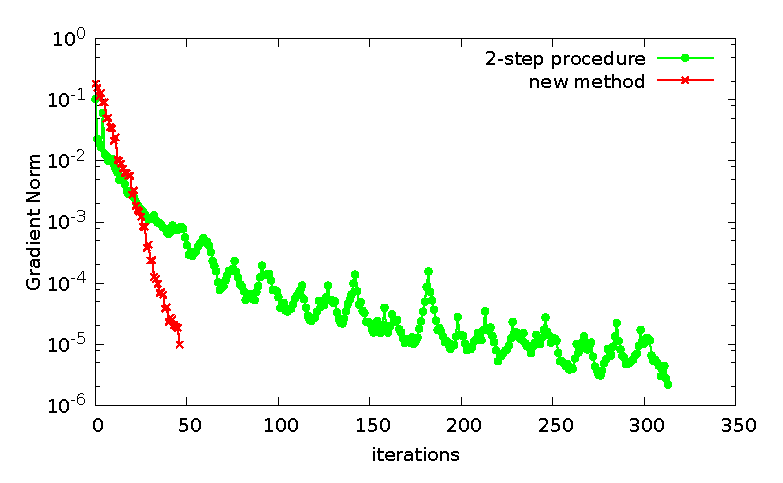
\includegraphics[width=0.5\textwidth]{convergence}
\caption{The maximun norm of energy gradient during the optimization. This is performed for 64 Si atoms with PBE exchange-correlation functional.}
\label{fig:convergence}
\end{figure}


\textbf{Results}
Our method is integrated with the CP2K package\cite{cp2kgeneral}, which uses the mixed Gaussian and plane wave method\cite{vandevondele2005quickstep}, and is an ideal platform for LS method. The optimization scheme is applied to systems with small band gap which are typically difficult for LS methods. Fig~\ref{fig:accuracy} shows the energy as a function of $R_c$ for several different systems: (a) CdSe of 768 atoms. (b) 64 water molecules, where each fragment is an atoms, and there are strong interaction and significant electron delocalization between fragments. (c) dimond Si of 512 atoms. We note that upon applying the filter $Q^x$ on the gradient, the final energy is no longer fully variational: the gradient is only zero in diretions that significantly change the energy. It also implies that the energy will depend on the optimization path. However, it is clear from Fig~\ref{fig:accuracy} that the energy converges to the DFT value as a function of cutoff, and the error mentioned is neglectable. 

\begin{figure}
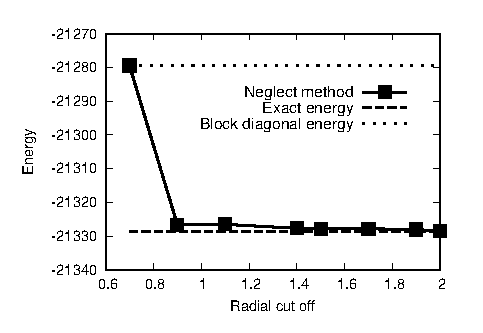
\includegraphics[width=0.35\textwidth]{CdSe}
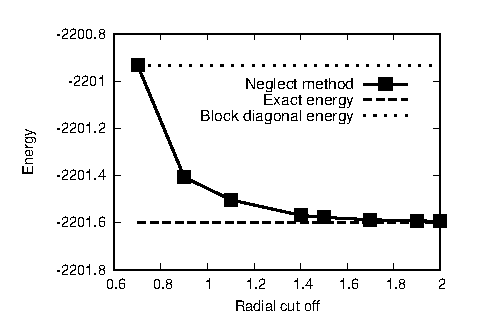
\includegraphics[width=0.35\textwidth]{H2O}
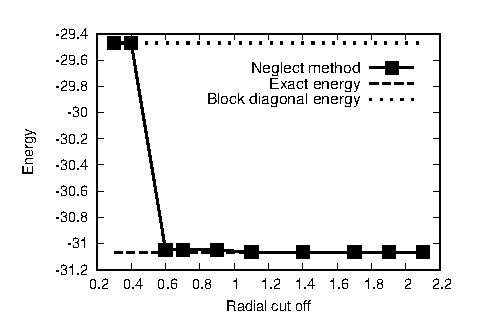
\includegraphics[width=0.35\textwidth]{Si}
\caption{The calculated energy as a function of the cutoff radii $R_c$. The systems involved are:(a) 128 water molecules with BLYP exchange-correlation functional and TZV2P basis set. Here each fragment is an atom, and covalent interactions happen between fragments. (b) 512 Silicon atoms with dimond lattice. PBE exchange-correlation functional and DZVP basis set are used. The convergence criteria used is $10^{-5}$.}
\label{fig:accuracy}
\end{figure}

\textbf{filtered directions}
Here we also discuss the physical meaning of the directions that are filtered out. The intuition from Eq~(\ref{eq:baddir}) implies that for each fragment $x$, each neighboring MO $|\psi_{yj}\rangle$ that only have a small portion outside of $x$ would contribute one problematic direction $P^x | \psi_{yj}\rangle$. And $Q^x$ should be a projector that removes all these directions, we assume MO $i$ on fragment $y$ that only have very small part outside of $x$, it will be denoted $xyi$, and the commen AOs of $x$ and $y$ fragments are denoted $xy\mu$, then $Q^x$ can be approximated as:

\bea
(Q^x)^{x\mu,x\nu} \approx S^{x\mu,x\nu} - T^{xy\mu}_{yi} (\sigma^{-1})^{xyi,xzj} T^{xz\mu}_{zj}
\label{eq:approxq}
\eea

where $\sigma^{xyi,xzj}$ is the overlap matrix,
\bea
\sigma^{xyi,xzj} = T^{xy\mu}_{xyi} S_{xy\mu,xz\nu} T^{xz\nu}_{xzj}
\eea
To verify this, we have calculated $Q^x$ using Eq~(\ref{eq:baddir}) and compare the result with that from Eq~(\ref{eq:qx}), for a small system of 4 HF molecules. The difference is within 1\% \new how to show?\old. However, although Eq~(\ref{eq:baddir}) gives a reasonable estimate of $Q^x$, it doesnot completely eliminate the problematic directions, and the optimization still suffers from convergence issues. Thus, although Eq~(\ref{eq:baddir}) is more intuitive and much easier to calculate, we cannot directly use it to optimize the energy.

The physical meaning of Eq~\ref{eq:approxq} is a modified orthogonality constrain for LMOs. Orthognality and locality has generally been considered as competing properties: strict orthogonality leads to decaying tails, and for LMOs no orthogonality constrains are imposed except for MOs within a fragment. However, this causes the convergence problem previously mentioned: LMOs without orthogonality tends to collapse. Although global orthogonality cannot be achieved, we suggest a local orthogonality constrain, that the projection of MOs onto each fragment $x$ should be orthogonal. Unlike the case for none-local MOs, not every physically meaningful state can be transformed into such state.

\textbf{linear performance}
To test the linear efficiency of the method, we compare the calculation with orbital transformation (OT) \cite{weber2008direct,vandevondele2003efficient}, which is one of most optimized cubic scaling DFT method. The calculation is done for CdSe with different system sizes. The radial cutoff is set to be 0.9 vdWR, which from Fig~\ref{fig:accuracy} is enough to accurately describe the system. The result is shown in Fig~\ref{fig:scaling}.

\begin{figure}
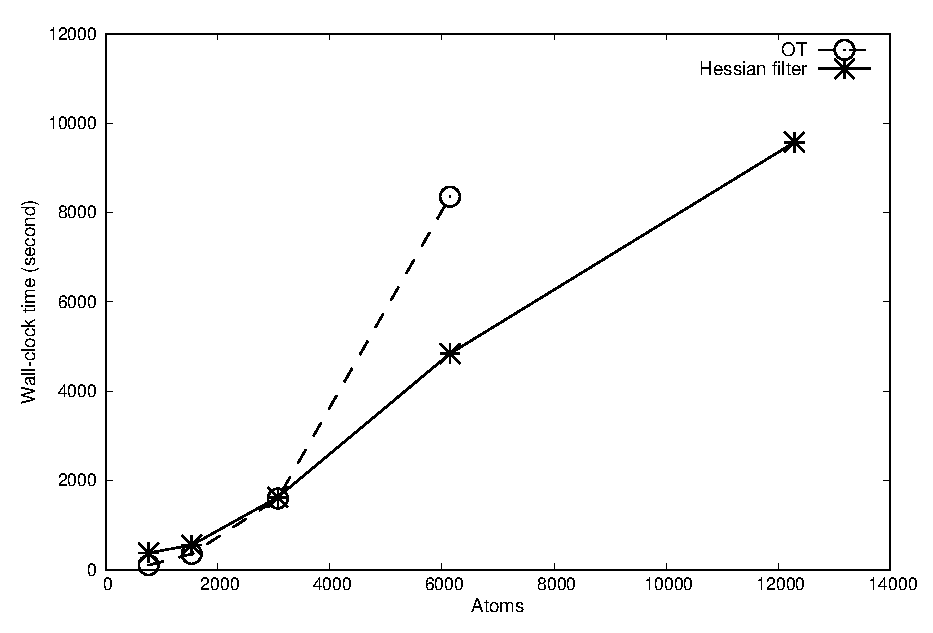
\includegraphics[width=0.45\textwidth]{timing}
\caption{Timing benchmark for the energy calculation of CdSe. The calculation is done on 256 cores. PBE exchange-correlation function is used and the radial cutoff is set to be 0.9 vDWR.}
\label{fig:scaling}
\end{figure}



\textbf{molecular dynamics}
To further demonstrate the accuracy of the force and energy calculation, we run a molecular dynamics (MD) simulation on a system of 62 water molecules with 2 H$^+$ atoms. The 2 protons will hop around through OH covalent bond breaking and reforming. We show in Fig~\ref{fig:md} the total energy during the MD run, compared to the that from OT calculation. 

\begin{figure}
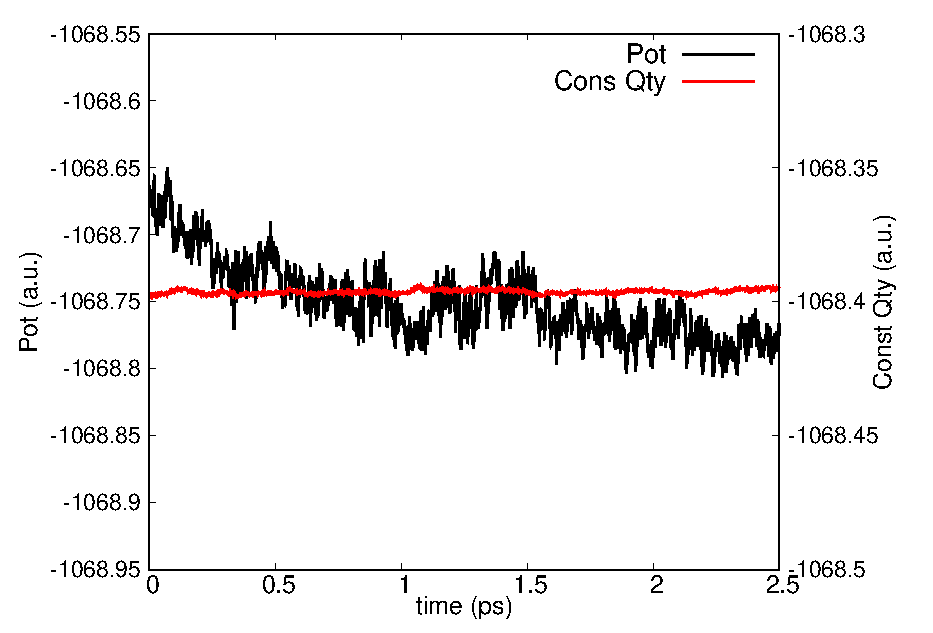
\includegraphics[width=0.45\textwidth]{const}
\caption{The total energy (kinetic plus potential) as a function of time, computed with linear scaling method and OT. Inset: the potential energy (Pot) and constant quantity (Const Qty) for linear scaling method.}
\label{fig:md}
\end{figure}

\textbf{Conclusion} We develop a new DFT method based on LMOs. The notorious convergence problem is avoided by identifying the small but none-zero eigenvalues of the Hessian. These directions are projected out from the gradient and the preconditioner, and the remaining gradient shows fast convergence with PCG. This projection can be understood as a relaxed orthogonality constrain for the LMOs. This method works even when the interaction and covalency between fragments are strong. We demonstrate the accuracy and efficiency of the method on systems like dimond silicon, CdSe. We also show a MD simulation in liquid water containing protons, and show that it can deal with systems where chemical reactions happen.


\textbf{Acknowledgments} 

The research was funded by the Natural Sciences and Engineering Research Council of Canada through the Discovery Grant. The authors are grateful to Compute Canada and McGill HPC Centre for computer time.

\bibliography{negref}

\end{document}
